\documentclass{article}
\usepackage{graphicx} % Required for inserting images
\usepackage{hyperref}
\usepackage{caption} % For custom captions
\usepackage{amsmath} 

\title{Theoretical Mechanics: Week Homework 3}
\author{Ekaterina Mozhegova}
\date{February 14, 2024}

\begin{document}

\maketitle

\section{Tools used for solving the tasks}

Python (sympy, matplotlib).

\section{Task 1}

\subsection{Link to the Code}

\href{https://colab.research.google.com/drive/1k7OYh1e7fFp5451cZUbvlRyAfRPKv4Xx?usp=sharing}{Colab}

\subsection{Task Description}

\noindent % Ensures no indentation to align with the left margin
\begin{minipage}{0.6\textwidth}
  You should find an absolute velocity and coriolis acceleration, and absolute acceleration of particle $M$ at the time $t=t_1$. 

  Needed variables:\\
  $OM=s_r(t)=f_3(t)=2t^3+3t$;\\
  $\phi(t)=f_2(t)=\frac{1}{24}\pi t^2$;\\
  $t_1=2,\ R=15$.
\end{minipage}%
\hfill % This ensures that there is no space between the minipages
\begin{minipage}{0.39\textwidth}
  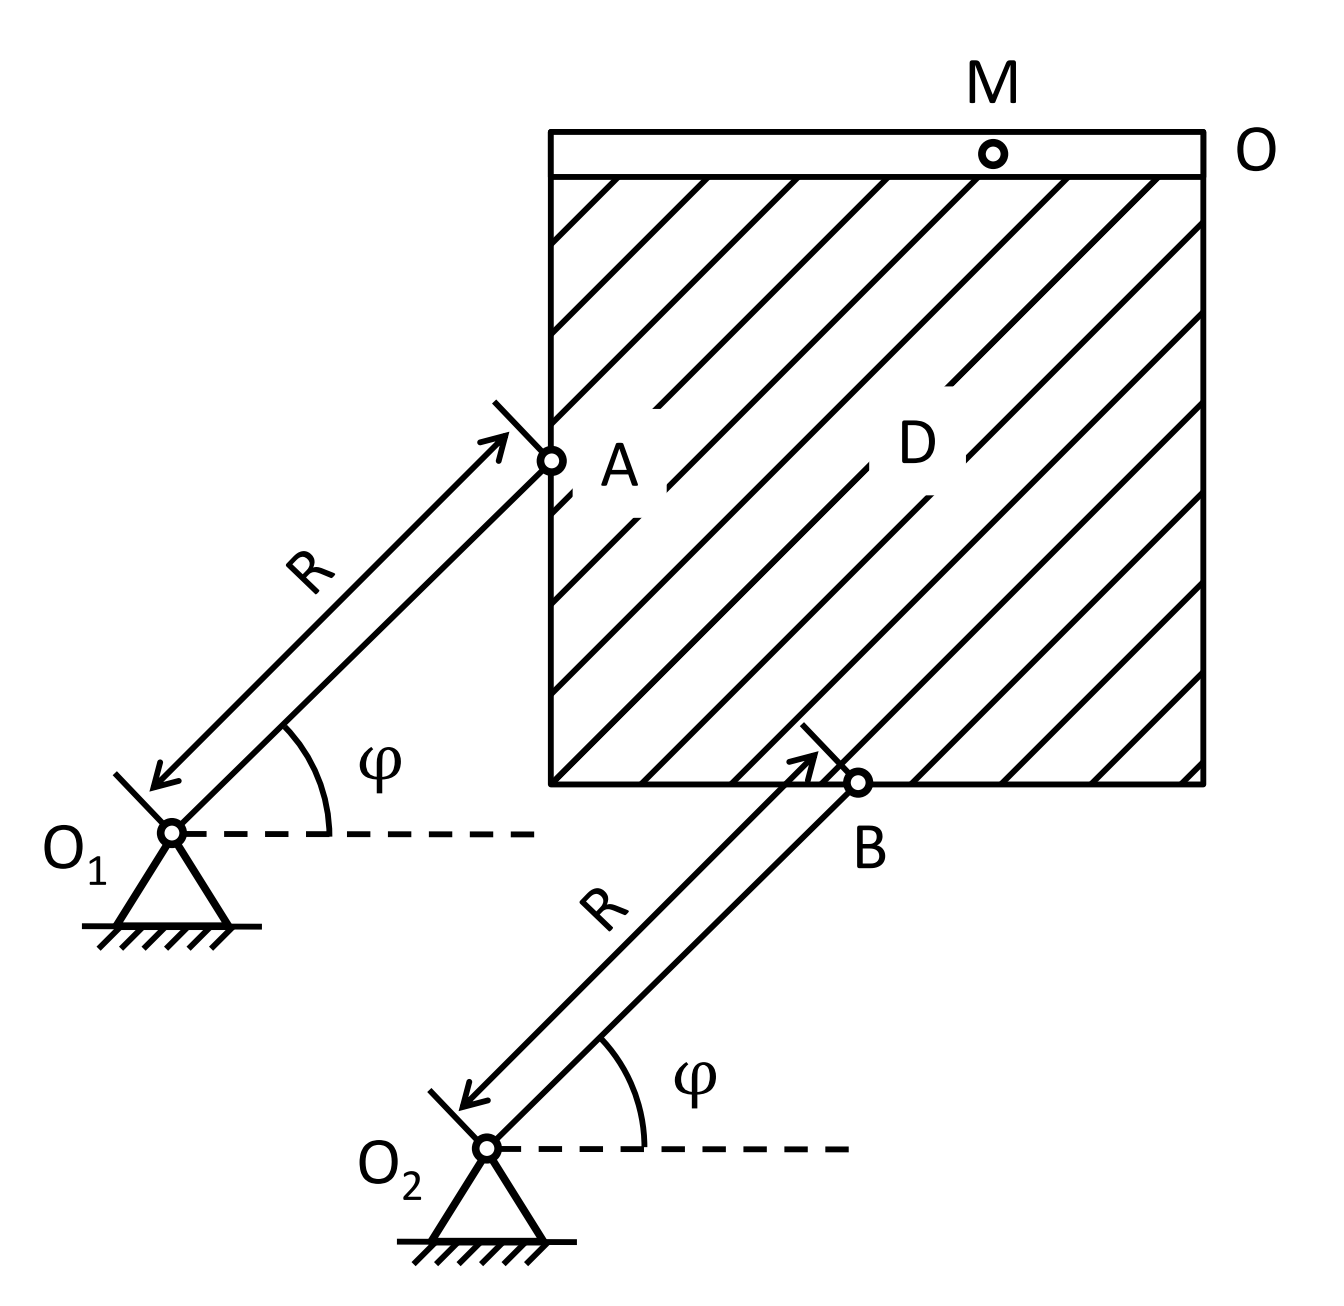
\includegraphics[width=\textwidth]{HW3_1.png} % Adjust the filename as necessary
  \captionof*{figure}{Task 1 (Yablonskii (eng) K-5)} % Corrected the caption to match the task
\end{minipage}

  
\subsection{Task explanation}

\begin{minipage}[t]{0.49\textwidth}

\begin{center} 
\underline{Velocity}
\end{center}
\raggedright
\textbf{1) Relative}

$v_{M}^{rel} = \dot s_r = 6t^2+3$
$v_{M}^{rel}(t_1) = 6(2^2)+3 = 27$\\

\textbf{2) Transport}

$\omega = \dot{\phi(t)} = \frac{\pi}{12} t$

$\epsilon = \dot{\omega} = \frac{\pi}{12}$

$\omega(t_1) = \frac{\pi}{6}$

$v_{M}^{tr}(t_1=2) = \omega(t_1=2) R = \frac{\pi}{6} \cdot 15 = \frac{5\pi}{2}$

\end{minipage}
\hfill
\begin{minipage}[t]{0.49\textwidth}

\begin{center} 
\underline{Acceleration}
\end{center}

No coriolis acceleration since the square body is in a translatory motion, it does not rotate.

$a_{M}^{rel} = \dot{v_{M}^{rel}} = 12t$

$a_{M}^{rel}(t_1) = \dot{v_{M}^{rel}(t_1)} = 24$


\end{minipage}

$\phi(t_1=2) = \frac{1}{24} \pi (2)^2 = \frac{\pi}{6}$

The velocity components and total velocity are given by:
\begin{align*}
    v_{M}^{y} &= v_{M}^{tr} \sin\left(\frac{\pi}{2} - \phi\right), \\
    v_{M}^{y}(t=t_1) &= v_{M}^{tr} \sin\left(\frac{\pi}{2} - \phi\right) = 5\frac{\pi}{2} \sin\left(\frac{\pi}{2} - \frac{\pi}{6}\right), \\
    v_{M}^{x} &= v_{M}^{tr} \cos\left(\frac{\pi}{2} - \phi\right) + v_{M}^{rel}, \\
    v_{M}^{x}(t=t_1) &= v_{M}^{tr} \cos\left(\frac{\pi}{2} - \phi\right) + v_{M}^{rel} = 5\frac{\pi}{2}\cos\left(\frac{\pi}{2} - \frac{\pi}{6}\right) + 27, \\
    V_{M}^{tot} &= \sqrt{v_{M}^{y}^2 + v_{M}^{x}^2} = 31.6661.
\end{align*}

Given constants:
\begin{align*}
a_{M}^{rel} &= 24, \\
\epsilon &= \frac{\pi}{12}, \\
\omega &= \frac{\pi}{6}.
\end{align*}

The acceleration components and total acceleration are:
\begin{align*}
a_{\tau}^{tr} &= \epsilon R, \\
a_{n}^{tr} &= \omega^2 R, \\
a_{M}^{y} &= a_{t} \sin\left(\frac{\pi}{2} - \phi\right) - a_{ntr} \sin(\phi), \\
a_{M}^{x} &= a_{M}^{rel} + a_{\tau}^{tr} \cos\left(\frac{\pi}{2} - \phi\right) + a_{n}^{tr} \cos(\phi), \\
a_{M}^{tot} &= \sqrt{a_{M}^{y}^2 + a_{M}^{x}^2} = 29.5555.
\end{align*}


\textbf{Answer: } $v_{M}^{tot} = 31.6661, a_{M}^{tot} = 29.5555, a_{M}^{cor} = 0$.


\section{Task 2}

\subsection{Link to the code}

\href{https://colab.research.google.com/drive/1K30VRx8tulT4y-6lVtZL8YNYCSKICuj9?usp=sharing}{Colab}

\subsection{Task Description}

\noindent
\begin{minipage}{0.6\textwidth}
      You should find:
      \begin{enumerate}
          \item simulate this mechanism (obtain all positions);
          \item Find absolute, transport and relative velocities and accelerations for $M$;
          \item Find $t$, when $M$ reaches $O$ point;
          \item draw plots $v_{rel},\ v_{tr},\ a_{tr},\ a_{rel},\ a$ respect to time.
      \end{enumerate}
      Needed variables:\\
      $\phi_e=f_1(t)=0.2t^3+t$;\\
      $OM=s_r=f_2(t)=5\sqrt{2}(t^2+t)$;\\
      $a=60,\ \alpha = 45$.
\end{minipage}
\hfill
\begin{minipage}{0.39\textwidth}
    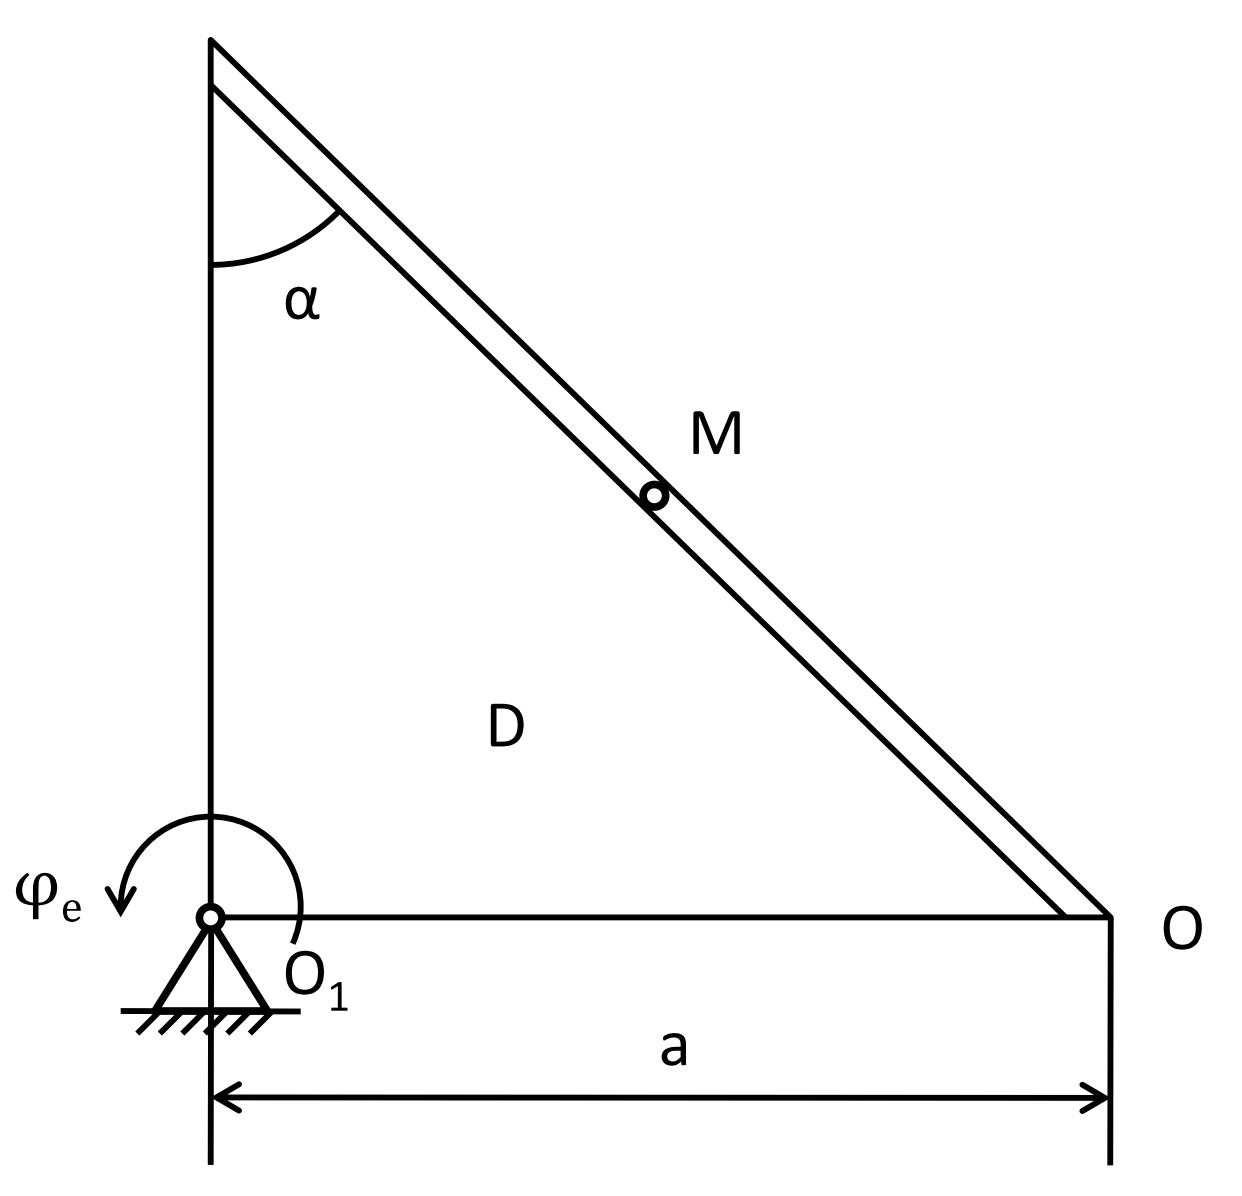
\includegraphics[width=\textwidth]{HW3_2.png}
    \captionof*{figure}{Task 2 (Yablonskii (eng) S6)}
\end{minipage}

\subsection{Task explanation}

First, let's calculate the time when M leaves the channel (i.e., when the point M travels the distance OA).

\[5\sqrt{2}(t^2 + t) = OA = 60\sqrt{2} \Rightarrow t = 3 \]

\textbf{1) Relative}

$v_{M}^{rel} = \dot{s}_r = 10\sqrt{2} t + 5\sqrt{2}$.

$a_{M}^{rel} = \ddot{s}_r = 10\sqrt{2}$\\
\textbf{2) Transport}

$\omega_e = \dot{\phi_e} = 0.6t^2 + 1$

$v_{M}^{tr} = \omega_e \cdot {MO_1}$

$a_{\tau}^{tr} = \dot{\omega_e} \cdot {MO_1} = \epsilon_e \cdot {MO_1}$

$a_{n}^{tr} = \omega_e^2 \cdot {MO_1}$\\
3) The Coriolis acceleration, \(a_{M}^{\text{cor}}\), is given by
\[
a_{M}^{\text{cor}} = 2 \mathbf{w}_{\text{tr}} \times \mathbf{v}_{M}^{\text{rel}}
\]

The Coriolis acceleration is directed to the center of rotation - $O_1$.

The directions of all velocities and accelerations is shown in the picture.

\begin{minipage}{0.8\textwidth}
    \includegraphics[width=\textwidth]{task2_solution.png}
    \captionof*{figure}{Task 2 (Yablonskii (eng) S6)}
\end{minipage}

\subsection{Plots}
\includegraphics[width=1.0\textwidth]{hw3_plots.png}

\subsection{Simulation}

\includegraphics[width=0.8\textwidth]{hw3_simulation1.png}

\includegraphics[width=0.8\textwidth]{hw3_simulation2.png}

\end{document}